% Customizable fields and text areas start with % >> below.
% Lines starting with the comment character (%) are normally removed before release outside the collaboration, but not those comments ending lines

% svn info. These are modified by svn at checkout time.
% The last version of these macros found before the maketitle will be the one on the front page,
% so only the main file is tracked.
% Do not edit by hand!
\RCS$Revision: 467027 $
\RCS$HeadURL: svn+ssh://tklijnsm@svn.cern.ch/reps/tdr2/notes/HIG-17-028/trunk/HIG-17-028.tex $
\RCS$Id: HIG-17-028_aux.tex 467027 2018-07-02 10:38:13Z tklijnsm $
%%%%%%%%%%%%% local definitions %%%%%%%%%%%%%%%%%%%%%
% This allows for switching between one column and two column (cms@external) layouts
% The widths should  be modified for your particular figures. You'll need additional copies if you have more than one standard figure size.
\newlength\cmsFigWidth
\ifthenelse{\boolean{cms@external}}{\setlength\cmsFigWidth{0.85\columnwidth}}{\setlength\cmsFigWidth{0.49\textwidth}}
\ifthenelse{\boolean{cms@external}}{\providecommand{\cmsLeft}{upper\xspace}}{\providecommand{\cmsLeft}{left\xspace}}
\ifthenelse{\boolean{cms@external}}{\providecommand{\cmsRight}{lower\xspace}}{\providecommand{\cmsRight}{right\xspace}}
%%%%%%%%%%%%%%%  Title page %%%%%%%%%%%%%%%%%%%%%%%%
\cmsNoteHeader{HIG-17-028} % This is over-written in the CMS environment: useful as preprint no. for export versions
% >> Title: please make sure that the non-TeX equivalent is in PDFTitle below
% \title{Combination of Higgs boson differential cross sections and limits on Higgs couplings with the 2016 dataset}
\title{Additional material for HIG-17-028}

% >> Authors
%Author is always "The CMS Collaboration" for PAS and papers, so author, etc, below will be ignored in those cases
%For multiple affiliations, create an address entry for the combination
%To mark authors as primary, use the \author* form
\author[cern]{The CMS Collaboration}

% >> Date
% The date is in yyyy/mm/dd format. Today has been
% redefined to match, but if the date needs to be fixed, please write it in this fashion.
% For papers and PAS, \today is taken as the date the head file (this one) was last modified according to svn: see the RCS Id string above.
% For the final version it is best to "touch" the head file to make sure it has the latest date.
\date{\today}

\abstract{Additional material: Simultaneous expected fit results for $\kappa_b$ and $\kappa_c$. One and two standard deviation contours are shown for the combined ($H \rightarrow \gamma\gamma$ and $H \rightarrow ZZ$) expectation, fixing the branching fractions to the values expected from the standard model. Also the corresponding one-dimensional scans of $\kappa_b$ and $\kappa_c$ are shown.}

% >> PDF Metadata
% Do not comment out the following hypersetup lines (metadata). They will disappear in NODRAFT mode and are needed by CDS.
% Also: make sure that the values of the metadata items are sensible and are in plain text:
% (1) no TeX! -- for \sqrt{s} use sqrt(s) -- this will show with extra quote marks in the draft version but is okay).
% (2) no %.
% (3) No curly braces {}.
\hypersetup{%
pdfauthor={M. Donega, T. Klijnsma, P. Musella},%
pdftitle={Combination of Higgs boson differential cross sections and limits on Higgs couplings},%
pdfsubject={CMS},%
pdfkeywords={differential cross sections, combination, Higgs coupling modifiers}}

\maketitle %maketitle comes after all the front information has been supplied
% >> Text
%%%%%%%%%%%%%%%%%%%%%%%%%%%%%%%%  Begin text %%%%%%%%%%%%%%%%%%%%%%%%%%%%%
%% **DO NOT REMOVE THE BIBLIOGRAPHY** which is located before the appendix.
%% You can take the text between here and the bibiliography as an example which you should replace with the actual text of your document.
%% If you include other TeX files, be sure to use "\input{filename}" rather than "\input filename".
%% The latter works for you, but our parser looks for the braces and will break when uploading the document.
%%%%%%%%%%%%%%%

\begin{figure}[hbtp]
  \begin{center}
    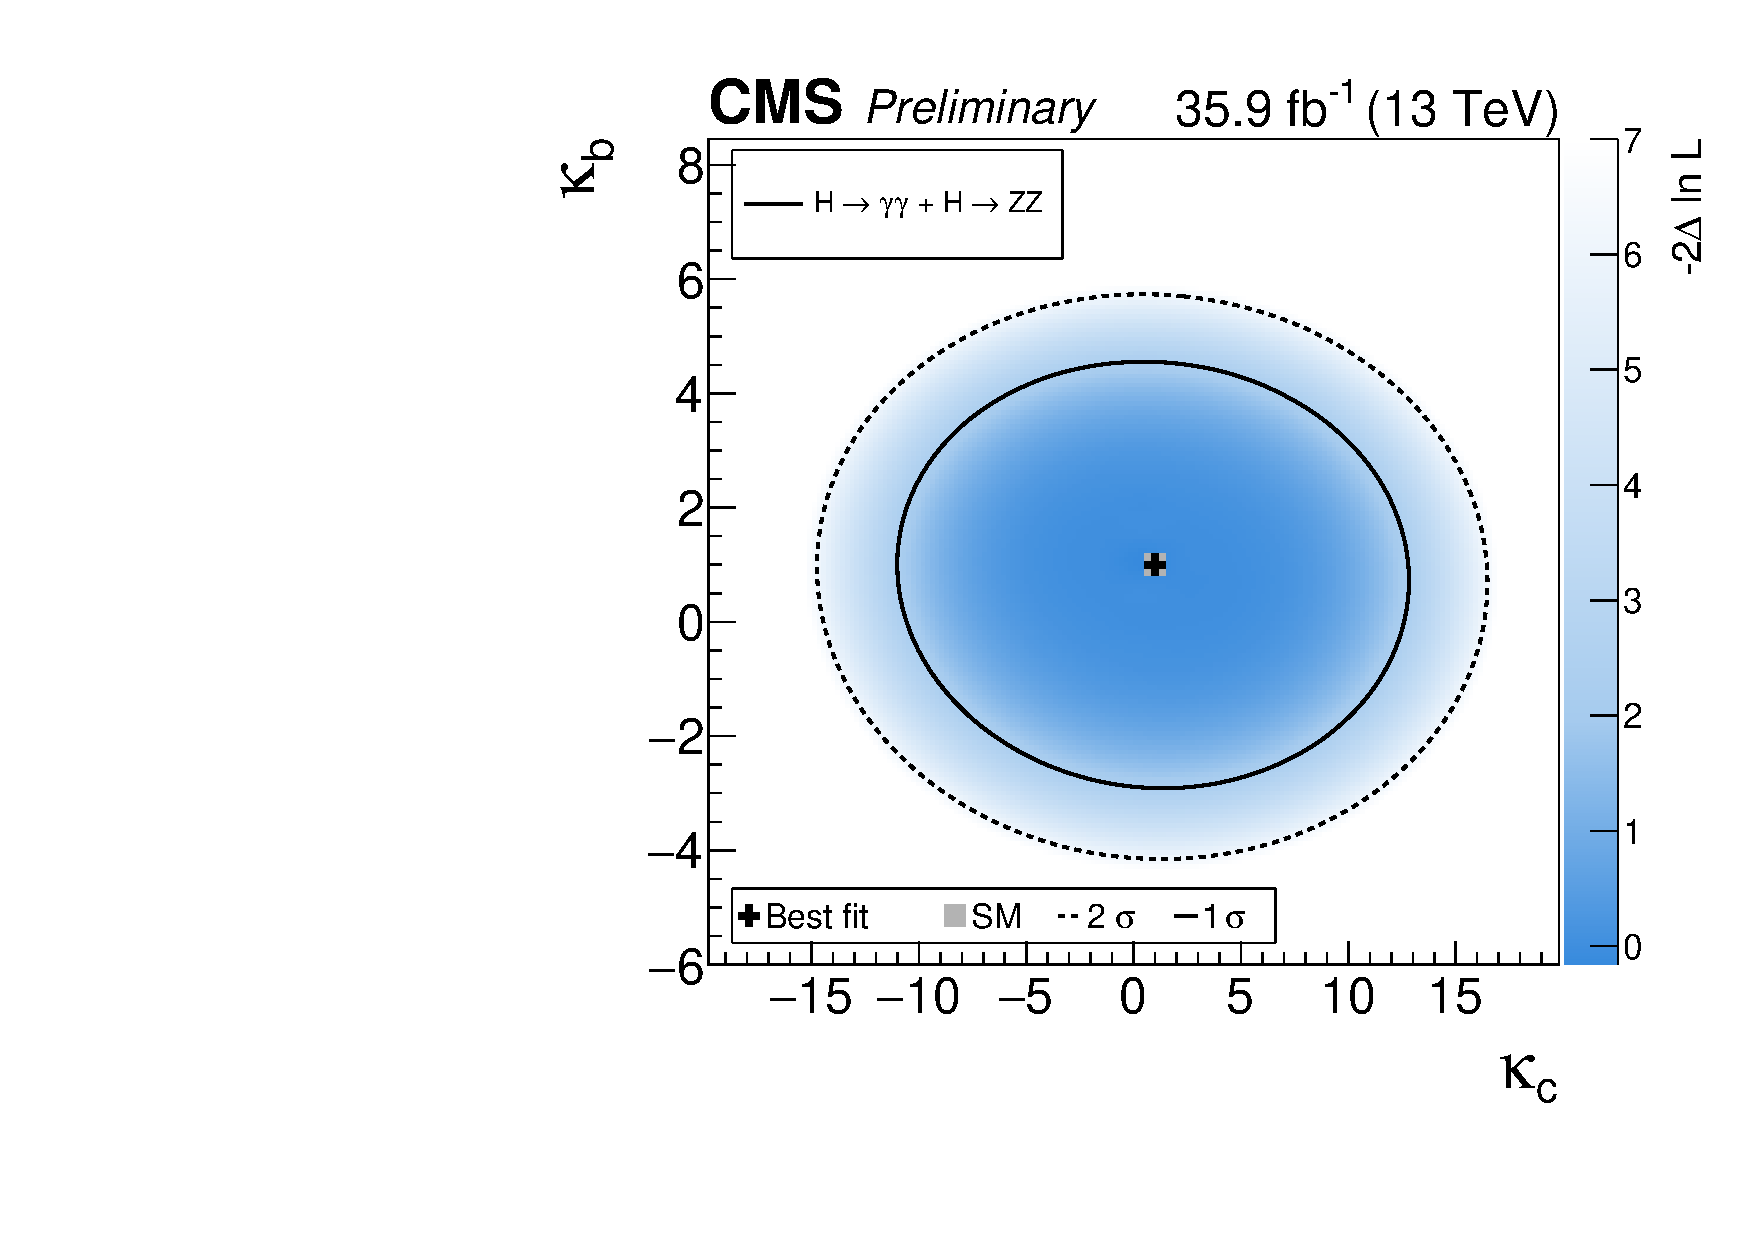
\includegraphics[width=0.9\linewidth]{img/supplementalmaterial/Fig1.pdf}
    % 
    \caption{
        Simultaneous expected fit results for $\kappa_b$ and $\kappa_c$. One and two standard deviation contours are shown for the combined ($H \rightarrow \gamma\gamma$ and $H \rightarrow ZZ$) expectation, fixing the branching fractions to the values expected from the standard model.
        }
    \label{fig:supplemental1}
  \end{center}
\end{figure}

\begin{figure}[hbtp]
  \begin{center}
    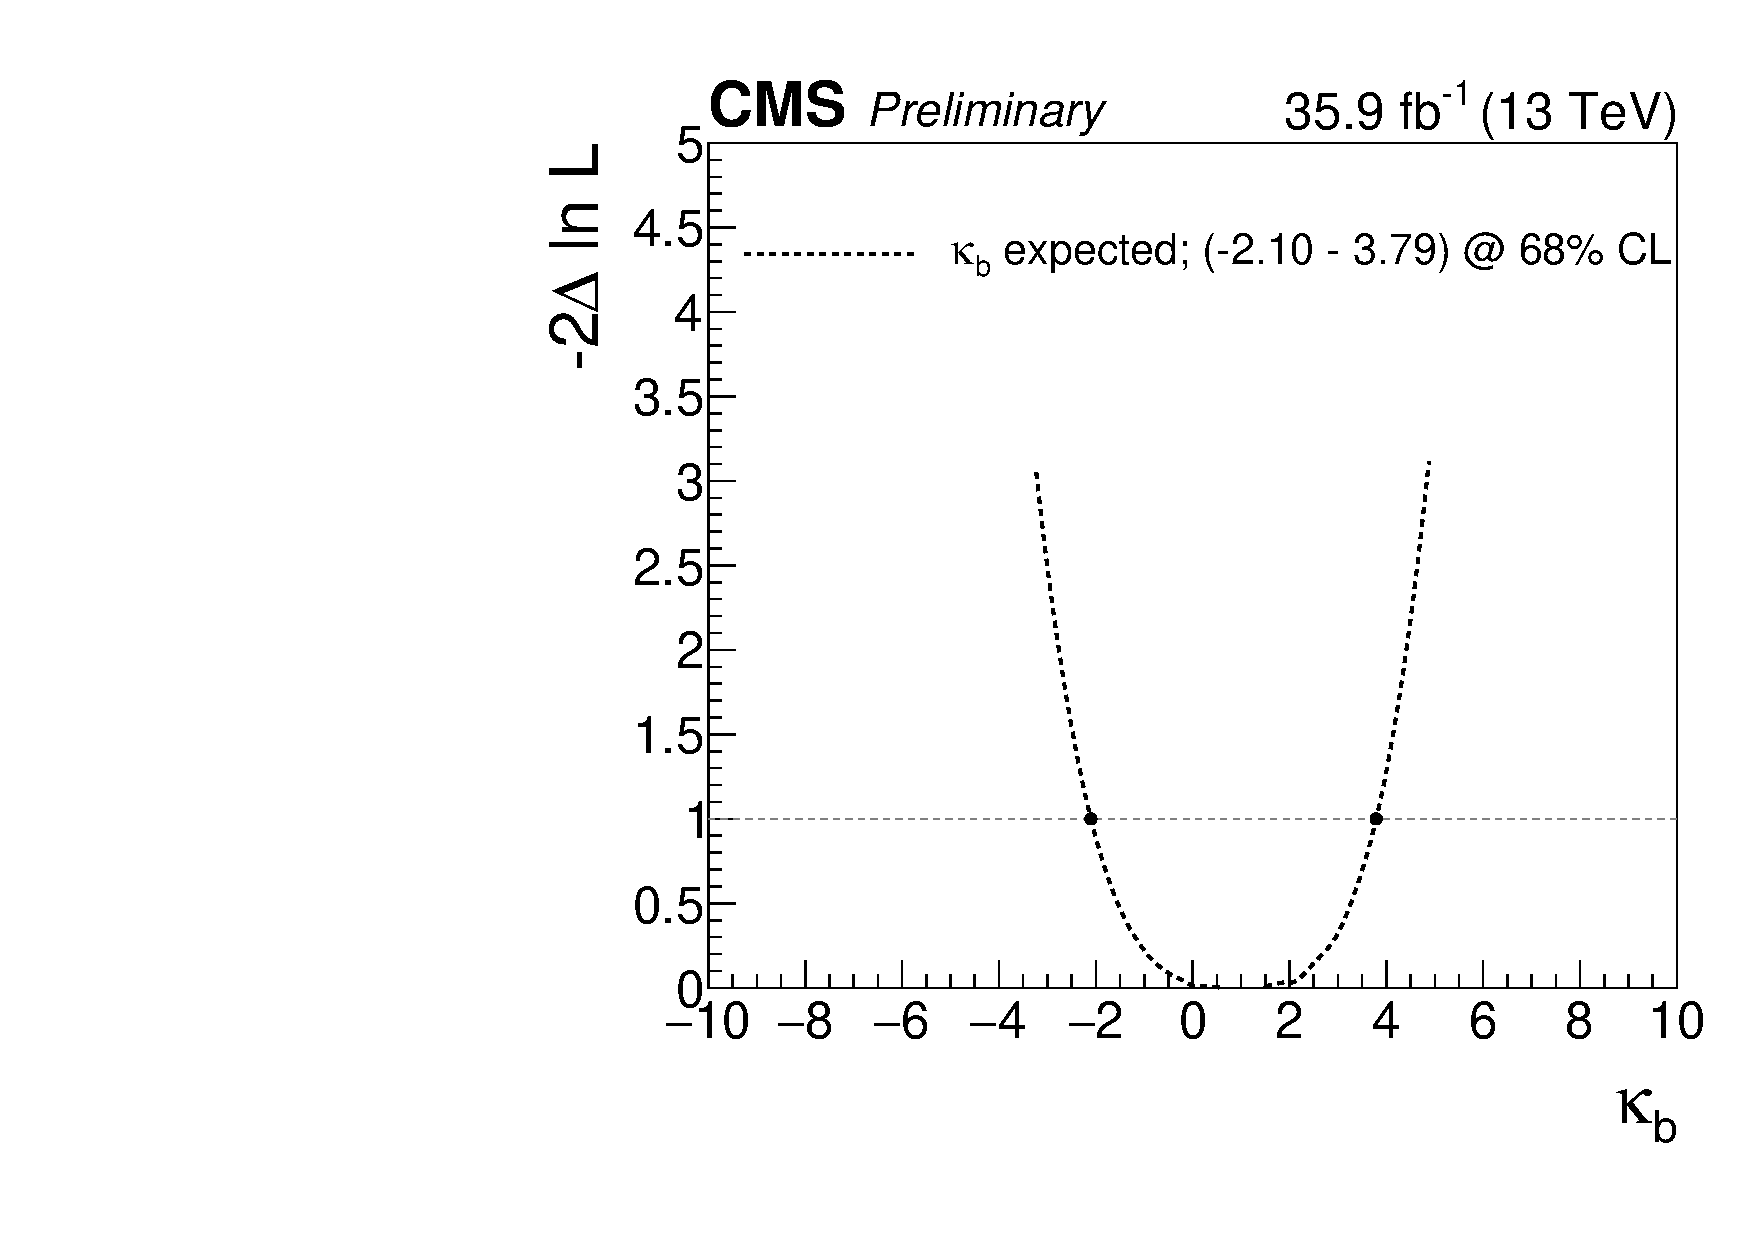
\includegraphics[width=0.9\linewidth]{img/supplementalmaterial/Fig2.pdf}
    % 
    \caption{
        Expected fit of $\kappa_b$ while profiling $\kappa_c$. The filled markers indicate the one standard deviation interval. The branching fractions were fixed to the values expected from the standard model.
        }
    \label{fig:supplemental2}
  \end{center}
\end{figure}

\begin{figure}[hbtp]
  \begin{center}
    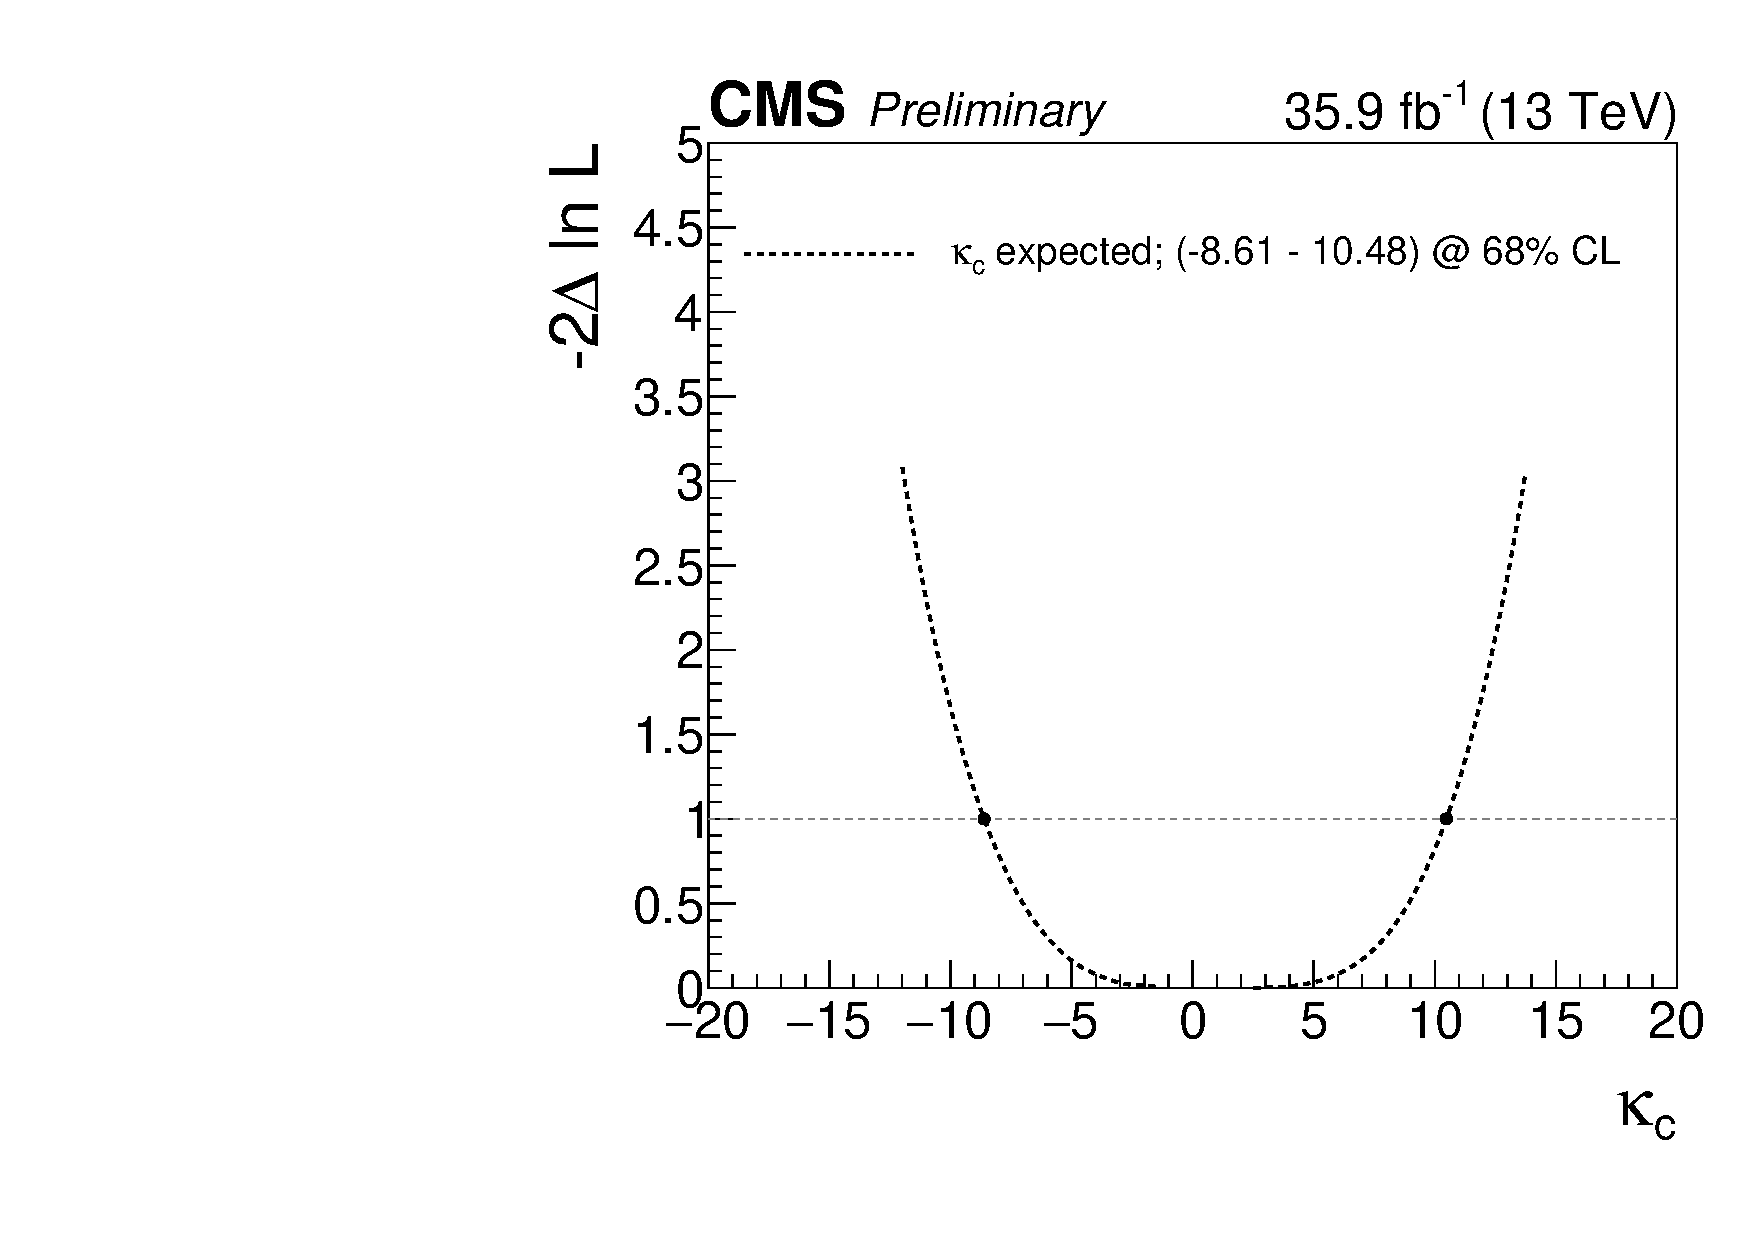
\includegraphics[width=0.9\linewidth]{img/supplementalmaterial/Fig3.pdf}
    % 
    \caption{
        Expected fit of $\kappa_c$ while profiling $\kappa_b$. The filled markers indicate the one standard deviation interval. The branching fractions were fixed to the values expected from the standard model.
        }
    \label{fig:supplemental3}
  \end{center}
\end{figure}

\clearpage

% ____________________________________________________________________________
%% **DO NOT REMOVE BIBLIOGRAPHY**
\bibliography{auto_generated}   % will be created by the tdr script.
